%
% Copyright (c) 2024
% Rémy Hubscher - <hubscher DOT remy AT gmail DOT com>
%
% This file may be distributed and/or modified under the terms of 
% the Apache v2 licence
% 

\documentclass{beamer}

\usetheme[shownavigation={false},  % true | false
          utbmlogo={LogoAAA.png},
          logo={logo.png},
          titlepageimage={titleimage.png},
          header=shortnav,          % fullnav | shortnav | utbm
          suiveur={Franck BERTAGNINI},
          dept={Formation FI (A)}
        ]{UTBM}

\usecolortheme{Terra}

\usepackage[francais]{babel}
\usepackage{datetime}  
\usepackage[T1]{fontenc}
\usepackage{lmodern}

\author{Rémy HUBSCHER} 

\begin{document}
  \title[Briefing Long — Risques Météo]{Phénomèmes météos dangereux pour l'aviation générale}
  \subtitle{Briefing Long — Risques Météo}
\date{\today} 

\begin{frame}[plain]
  \titlepage
\end{frame}

\begin{frame}{Objectifs}
  Étudier l'impact des phénomènes météo sur la sécurité des vols
\end{frame}

\begin{frame}{Utilité}
  \begin{itemize}
    \item Voler en toute sécurité ; \pause
    \item Connaître les manœuvres de protection ; \pause
    \item Déceler les situations à risque ; \pause
    \item Renoncer quand le risque est trop grand ;
  \end{itemize}  
\end{frame}

\begin{frame}{Questions}
  \begin{itemize}
    \item Qu'est-ce que la température du point de rosée ? \pause
    \item Qu'est-ce que le carburateur ? \pause
    
    \item Quel est le taux d'humidité d'une atmosphère à 20°C dont le point de rosée est à 17°C ? \pause
    \item Quelle est la base des nuages d'une même atmosphère ?
  \end{itemize}  
\end{frame}

\begin{frame}{Thème}
  \tableofcontents
\end{frame}

\begin{frame}{Rapport}
  \begin{itemize}
    \item Avez-vous entendu parler de brouillard givrant ?
    \item Avez-vous vu de grosses averses ou orage de grêle ?
    \item Avez-vous fait du vélo par grand vent ?
    \item Savez-vous qu'elle est l'heure la plus froide d'une journée ?
    \item \href{https://www.youtube.com/watch?v=zIhQlqZ7UN8}{Vidéo tempête dans le Jura}
  \end{itemize}  
\end{frame}


\section{Brumes et brouillards}
\begin{frame}{Brumes et brouillards}
  \LARGE{Brumes et brouillards}
\end{frame}

\begin{frame}{Brumes et brouillard}
  \begin{itemize}
    \item La Brume : Suspension, dans l’atmosphère, de microscopiques gouttelettes d’eau, réduisant la visibilité entre 1 et 5 km. \pause
    \item La Brume sèche : particules solides (sable et poussières) dans l'air non saturé en humidité \pause
    \item Le Brouillard : Suspension dans l'air de petites goutelettes d'eau ou de glace, réduisant la visibilité à moins de 1 km. ; \pause
    \item Le Brouillard se forme par refroidissement d'une masse d'air humide : Saturation puis Condensation.
  \end{itemize}
\end{frame}

\begin{frame}{Brumes et brouillard}
  On distingue différents types de brouillard :
  \pause
  \begin{itemize}
    \item de rayonnement : réchauffement de la rosée du matin \pause
    \item d'évaporation : arrivée d'air froid et sec sur une étendue d'eau \pause
    \item d'advection : arrivée d'air chaud et humide sur un sol froid \pause
    \item de pente : soulèvement d'air humide \pause
    \item de mélange : de 2 masses d'air de températures différentes par brassage
  \end{itemize}
\end{frame}


\section{Givrage carburateur} 
\begin{frame}{Givrage carburateur}
  \LARGE{Le Carburateur : Risque de givrage}
\end{frame}
\begin{frame}{Givrage carburateur} 
  Sur les moteurs à pistons à carburateur, il existe un risque de
  givrage du papillon de gaz.

  \pause
  \begin{figure}
    \centering
    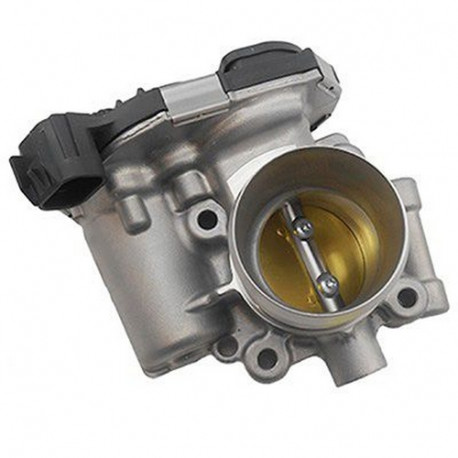
\includegraphics[scale=0.5]{images/papillon-gaz.jpg}
  \end{figure}

  \pause
  Cela est dû à l'effet Venturi.
\end{frame}

\begin{frame}{L'effet Venturi}
  \begin{itemize}
    \item En passant dans le carburateur, l'air aspiré par le moteur accélère \pause
    \item Cette acceleration créé un dépression ; \pause
    \item Cette depression fait baisser la température ; \pause
    \item Si la température baisse dans un air humide, il y a un risque de givrage moteur.
  \end{itemize}
\end{frame}

\begin{frame}{Givrage carburateur} 
  \begin{figure}
    \centering
    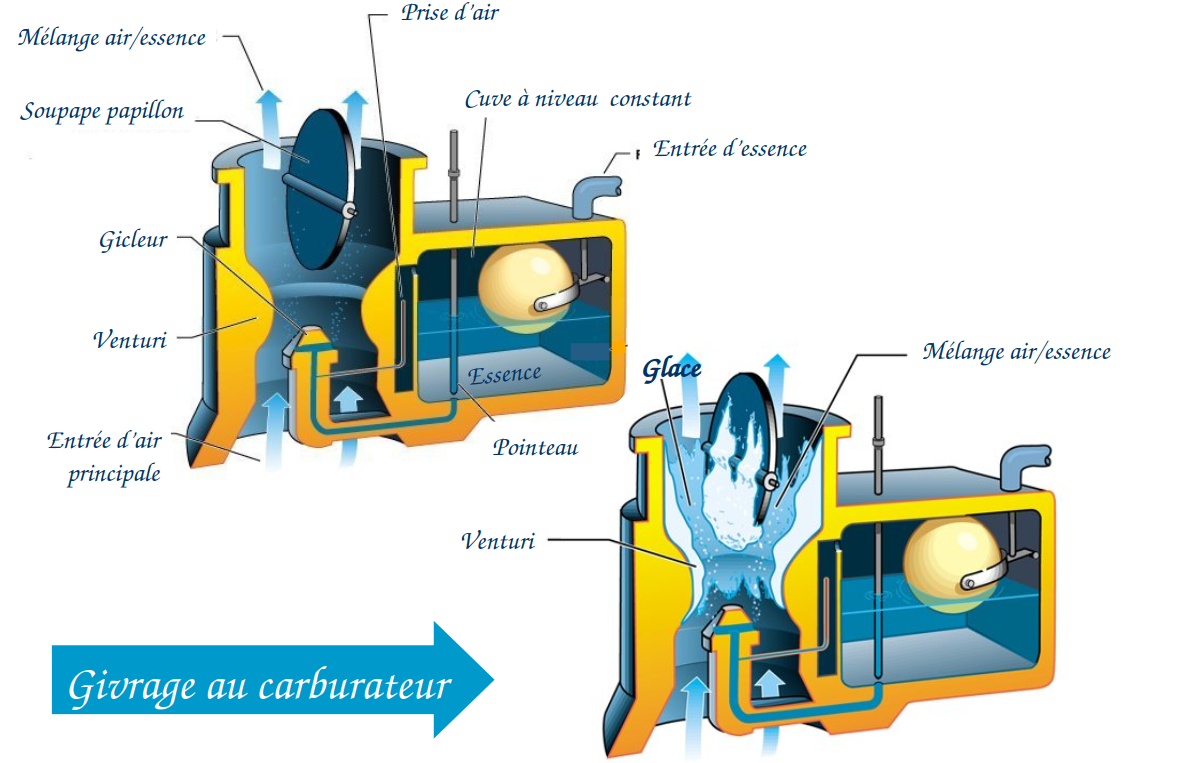
\includegraphics[scale=1]{images/carburateur.png}
  \end{figure}
\end{frame}


\begin{frame}{Zone de risque de givrage}
  \begin{figure}
    \centering
    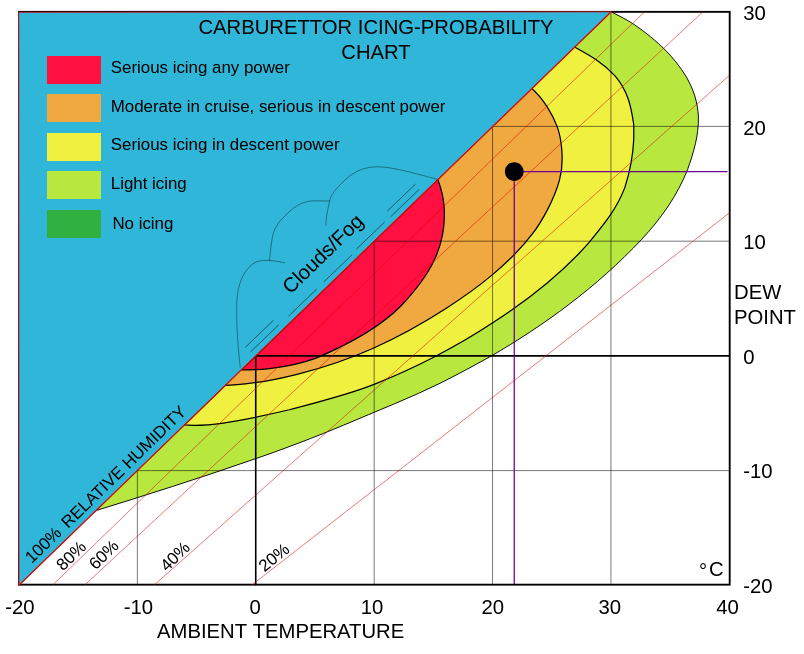
\includegraphics[scale=1.5]{images/icing.png}
  \end{figure}
\end{frame}

\begin{frame}{Contre mesures}
  Pour éviter le givrage :\pause
  \begin{itemize}
    \item On ne vole pas dans les nuages ; \pause
    \item On allume la réchauffe lors d'une réduction des gaz et en tour de piste \pause
    \item En croisière, une perte de tours est un signe de début de givrage. \pause
    \item Au démarrage, on peut également givrer, mettre la réchauffe à l'arrêt peut-être nécessaire.
  \end{itemize}
  
\end{frame}


\section{Givrage cellule}
\begin{frame}{Givrage cellule}
  \LARGE{Risque du Givrage de la Cellule}
\end{frame}

\begin{frame}{Givrage cellule}
  C'est la formation, plus ou moins rapide, d'un dépôt de glace sur des parties de l'avion.

  \pause
  Ce dépôt de glace :   \pause

  \begin{enumerate}
    \item Alourdit l'avion \pause
    \item Modifie l'écoulement de l'air autour de l'avion et influe sur les performances \pause
    \item peut bloquer les gouvernes, volets et sondes Pitot, ... \pause
    \item peut étouffer le moteur (lors du givrage carburateur ou givrage du filtre à air)
  \end{enumerate}
\end{frame}

\begin{frame}{Givrage cellule au sol}
  Il est possible que l'aile se couvre de glace au sol
  \pause
  \begin{enumerate}
    \item Dans un air humide brouillard ; \pause
    \item Les ailes des avions métaliques pleines de carburant froid ; \pause
    \item Cela peut se produire au point d'attente en vol de nuit
  \end{enumerate}
\end{frame}

\begin{frame}{Givrage cellule au sol}
  Une couche de 0.5cm sur toute la surface de l'aile, va augmenter le poids de plusieurs dizaines de kilos et modifier l'écoulement de l'air.
  \pause
  \begin{figure}
    \centering
    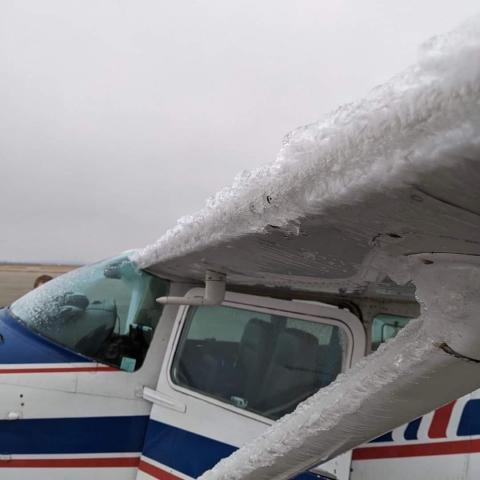
\includegraphics[scale=0.5]{images/GIVRAGE.jpg}
  \end{figure}
  
  La vitesse de décrochage augmente
\end{frame}

\begin{frame}{Givrage cellule en vol}
  En passant dans un nuage, l'humidité froide en suspension trouve un
  élément où s'accrocher notamment avant la vitesse de déplacement.
  \pause
  
  La prise de glace est très rapide, peut boucher la visibilité et
  faire chuter rapidement l'avion et ce même hors des nuages.
  \pause
  \begin{figure}
    \centering
    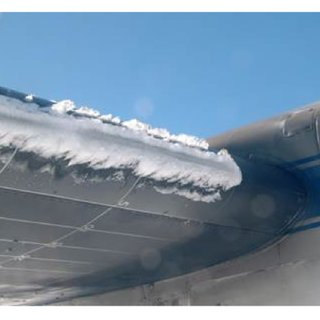
\includegraphics[scale=0.5]{images/accretion.jpg}
  \end{figure}
  
\end{frame}

\begin{frame}{Catégorie de givrage : Le givre}
  Le Givre
  \pause

  \begin{enumerate}
    \item Lorsque l'avion vole dans une zone de pluie surfondue (eau liquide entre 0 et -15°C) \pause
    \item Ce phénomène se produit notamment au niveau d'un front froids. \pause
    \item Risque indiqué sur les cartes TEMSI et dans les SIGMET.
  \end{enumerate}
\end{frame}

\begin{frame}{Catégorie de givrage : Le verglas}
  Le Verglas
  \pause

  \begin{enumerate}
    \item Congélation de pluie ou de bruine \pause
    \item Surfondue ou non, hors ou dans les nuages. \pause
    \item Dépôt transparent qui se forme rapidement pouvant atteindre des épaisseurs importantes sur toute la surface de l'avion.
  \end{enumerate}
\end{frame}

\section{Le cumulonimbus}
\begin{frame}{Le cumulonimbus}
  \LARGE{Le cumulonimbus a.k.a CB ou Cunimb}
\end{frame}

\begin{frame}{Le cumulonimbus}
  Les cumulonimbus sont des très gros nuages qui montent jusqu'à la stratosphère.

  \pause

  C'est le nuage le plus dangeureux pour l'aviation.

  \pause

  Il se forme en avant des fronts froids ou après un fort échauffement du sol.

  \pause
  
  Il est nécessaire de les contourner largement même pour les gros avions de ligne.
\end{frame}

\begin{frame}{Cumulonimbus supercellulaire}
  \begin{figure}
    \centering
    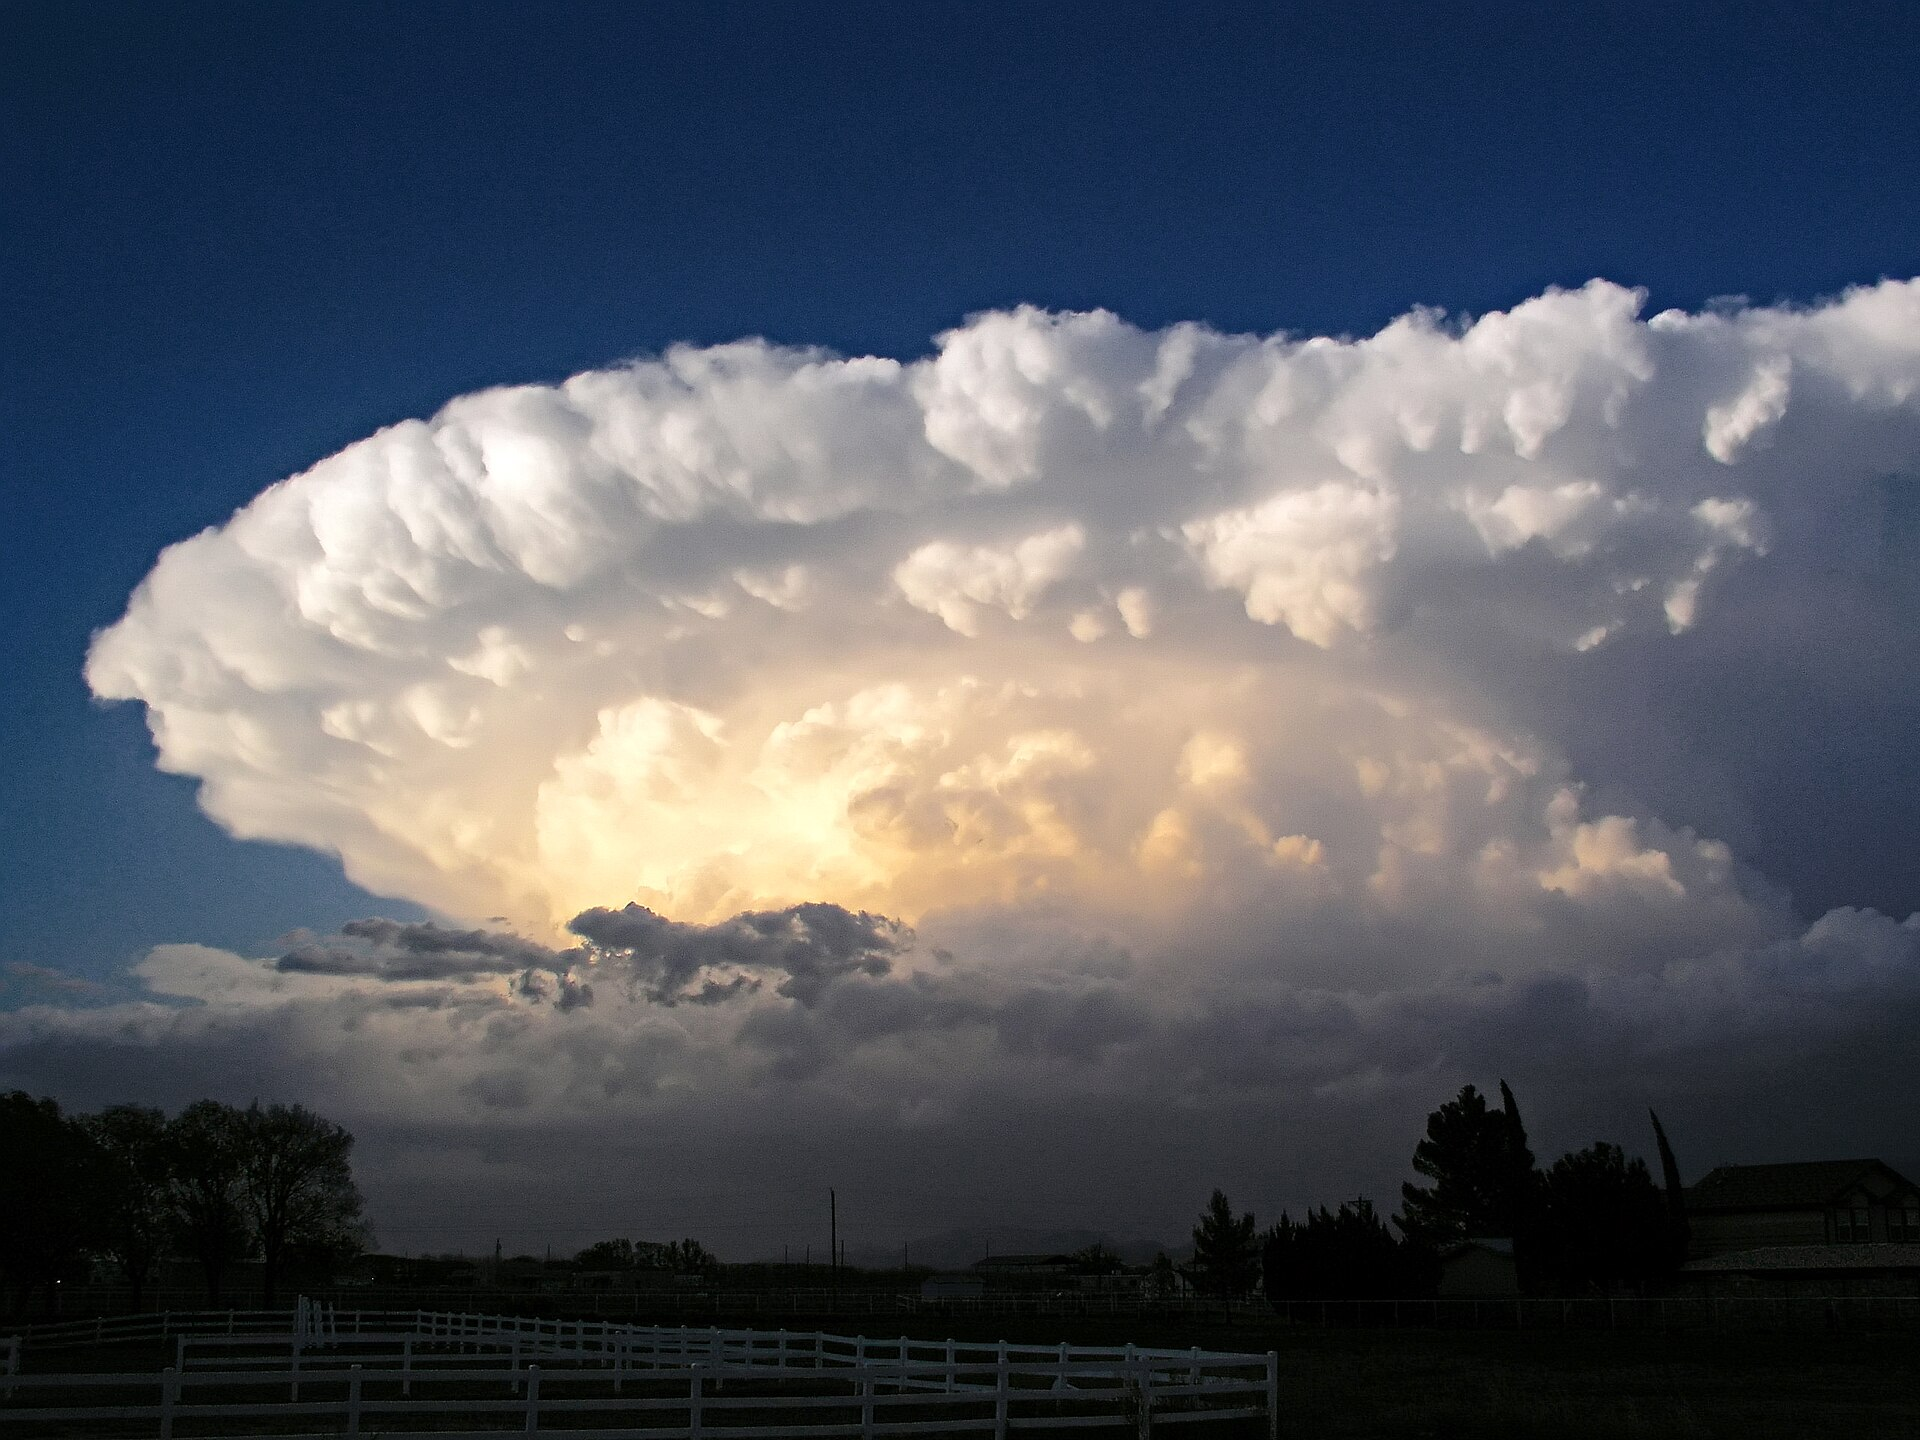
\includegraphics[scale=0.16]{images/Chaparral.jpg}
  \end{figure}
\end{frame}

\begin{frame}{Formation des Cb}
  Il provoque :
  \begin{itemize}
    \item Du vent : Très violent et très irrégulier. La direction peut changer brutalement. \pause
    \item Des grains : Vents violents accompagnés d'averses intenses. \pause
    \item Des averses de pluie : Réduisent complément la visibilité. \pause
    \item De la turbulence : Les vents verticaux peuvent avoisiner les 90 km/h. \pause
    \item De la grêle : Elle réduit la visibilité et peut endommager la cellule de l'avion. \pause
    \item De la foudre : Elle peut endommager les moyens de radionavigation.
  \end{itemize}
\end{frame}

\begin{frame}{Cisaillement de vent}
  \begin{figure}
    \centering
    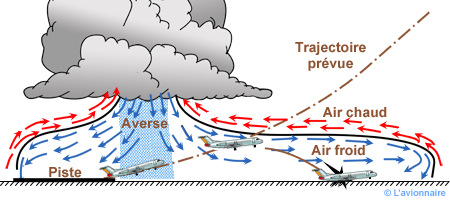
\includegraphics[scale=0.7]{images/cisaillement.png}
  \end{figure}
\end{frame}

\section{Les phénomènes météorologiques locaux}

\begin{frame}{Les phénomènes météorologiques locaux : Le Foehn}

  Le Foehn
  \pause
  
  Phénomène spécifique aux régions montagneuses.

  \pause

  Il s'agit du franchissement d'un obstacle (montagne) par une masse d'air humide.

  \pause

  \begin{figure}
    \centering
    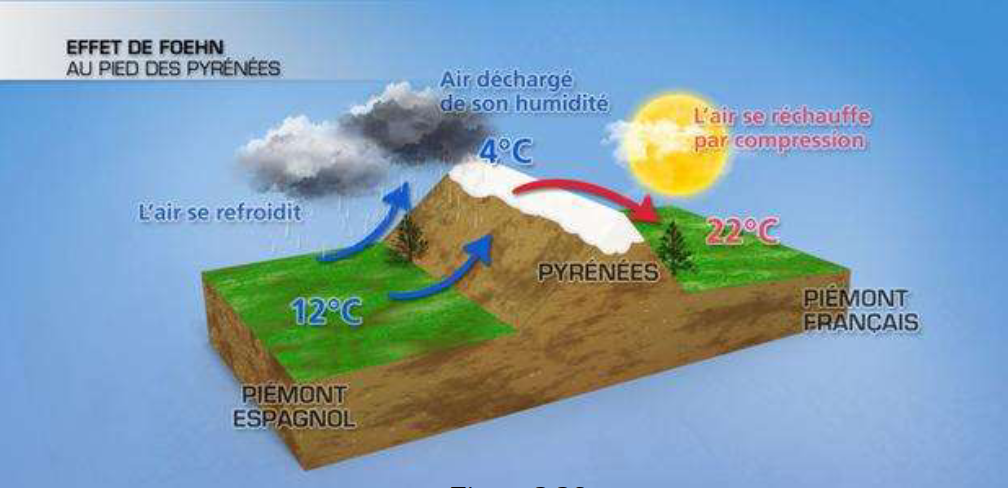
\includegraphics[scale=1]{images/foehn.png}
  \end{figure}

\end{frame}

\begin{frame}{Les phénomènes météorologiques locaux : La Brise}
  La Brise
  \pause
  
  Phénomène spécifique aux régions de lac, vallées, montagne ou de mer.

  \pause

  Provoqué par les différences de températures entre les masses d’air
  dans les basses couches de la troposphère et il suit un cycle
  jour/nuit.

\end{frame}

\begin{frame}{La Brise de Mer / La Brise de Terre}
  La Brise de Mer
  \pause
  
  \begin{figure}
    \centering
    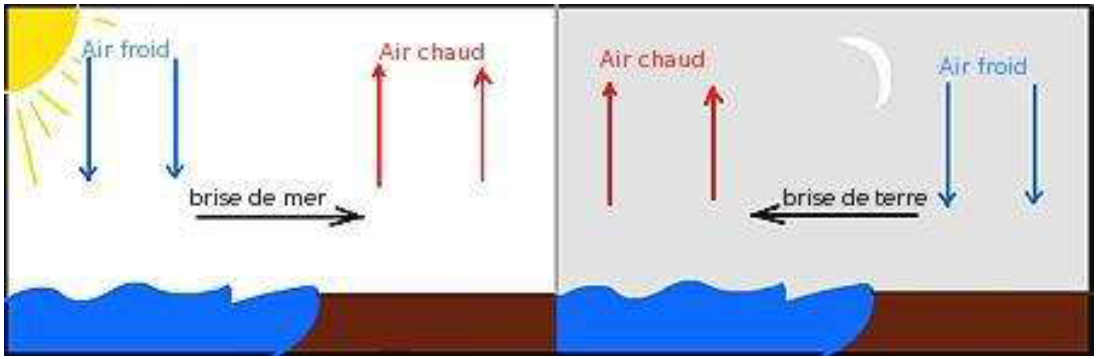
\includegraphics[scale=1]{images/brise-mer.png}
  \end{figure}

  \pause
  Le jour, le sol se rechauffe plus vite que la mer : brise de mer

  \pause du milieu de matinée à la fin d'après-midi

  \pause
  La nuit, le sol se refroidit plus vite que la mer : brise de terre

  \pause en fin de soirée.

\end{frame}

\begin{frame}{La Brise de Pente}
  La Brise de Pente
  \pause
  

  \begin{figure}
    \centering
    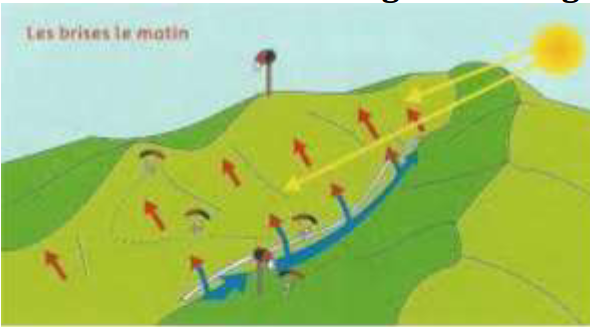
\includegraphics[scale=1]{images/brise-montagne-matin.png}
  \end{figure}

  \pause
  Le matin, l'air au contact des versants ensoleillés s'échauffe et s'élève le long des pentes

  \pause le vent s'établit remontant la vallée

\end{frame}

\begin{frame}{La Brise de Pente}
  
  \begin{figure}
    \centering
    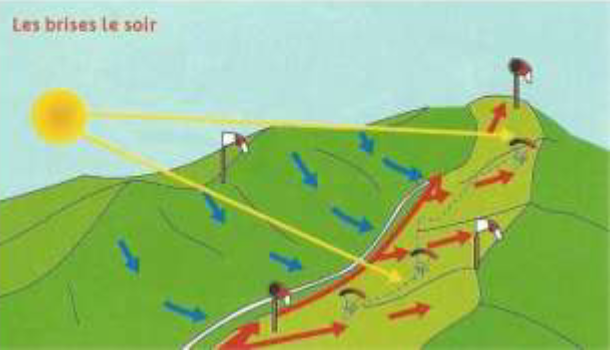
\includegraphics[scale=1]{images/brise-montagne-soir.png}
  \end{figure}

  \pause
  Le soir, le phénomène inverse se produit, descendant les pentes à l'ombre

  \pause le vent s'établit descendant la vallée

\end{frame}

\begin{frame}{La Turbulence}
  La Turbulence
  \pause
  
  \begin{itemize}
    \item Sous les cumulus \pause
    \item Au contact de deux masses d'air \pause
    \item En air clair : Les CAT en présence de forts gradients de température et de pression \pause
      
      signalée sur les cartes météo quand c'est possible
  \end{itemize}
\end{frame}

\begin{frame}{Les ondes orographiques}
    Les ondes orographiques
  \pause

  \begin{figure}
    \centering
    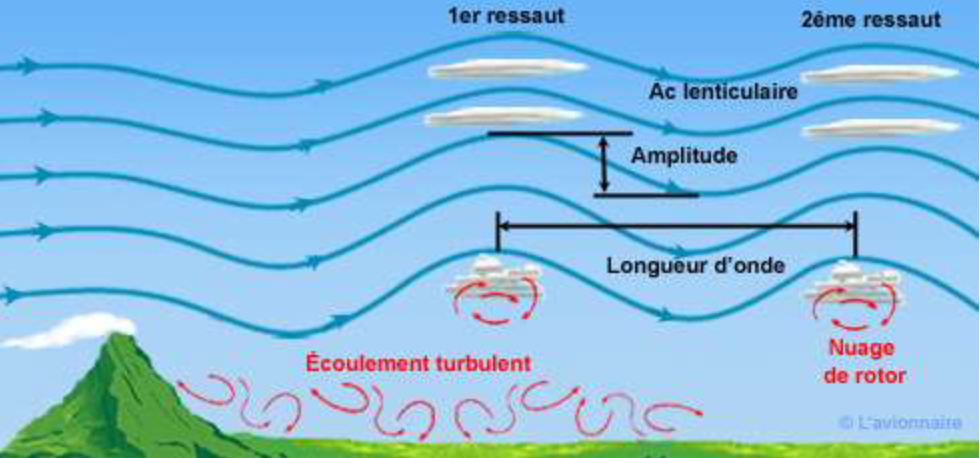
\includegraphics[scale=1]{images/orographique.png}
  \end{figure}
\end{frame}

\begin{frame}{Le jet stream}

  Les Jet Stream sont des courants d'air très rapides de quelques
  centaines de kilomètres de large et de seulement quelques kilomètres
  d'épaisseur.

  \pause

  Ils sont situés à environ 10 kms d'altitude.

  \pause
  
  \begin{figure}
    \centering
    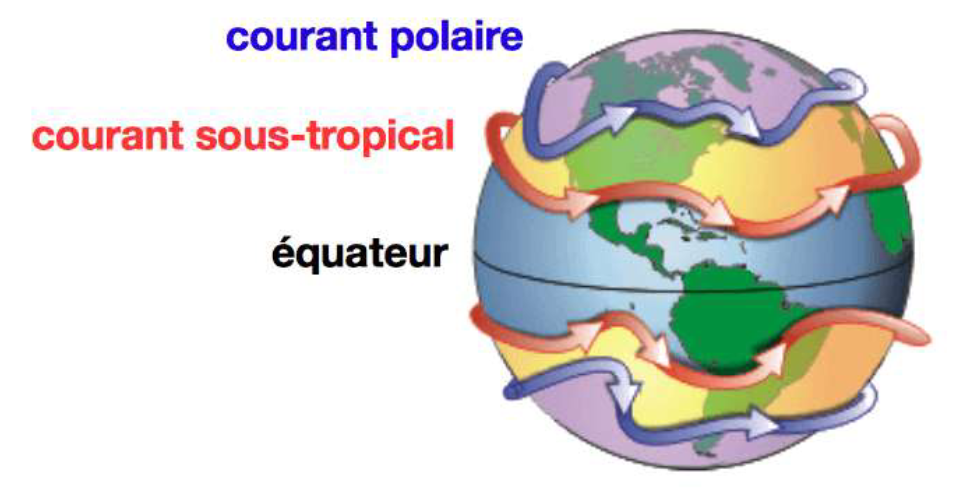
\includegraphics[scale=1]{images/jet-stream2.png}
  \end{figure}

  \pause

  La vitesse des vents est d'environ 200 à 300 kmh.
  
\end{frame}

\begin{frame}{Le jet stream}

  Le Jet-stream entoure le globe terrestre, et souffle d’Ouest en Est
  selon la rotation de la terre. Il se situe au niveau de la
  tropopause, à la jonction des cellules de convection.
  
  \begin{figure}
    \centering
    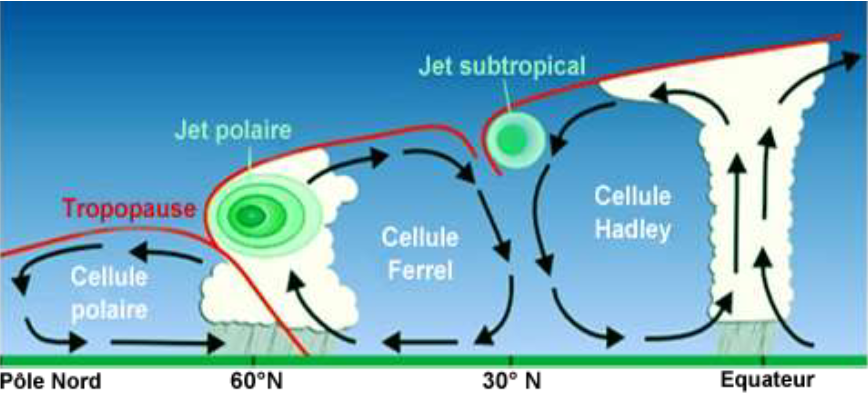
\includegraphics[scale=1]{images/jet-stream1.png}
  \end{figure}
\end{frame}

\begin{frame}{Les vents locaux}
  
  \begin{figure}
    \centering
    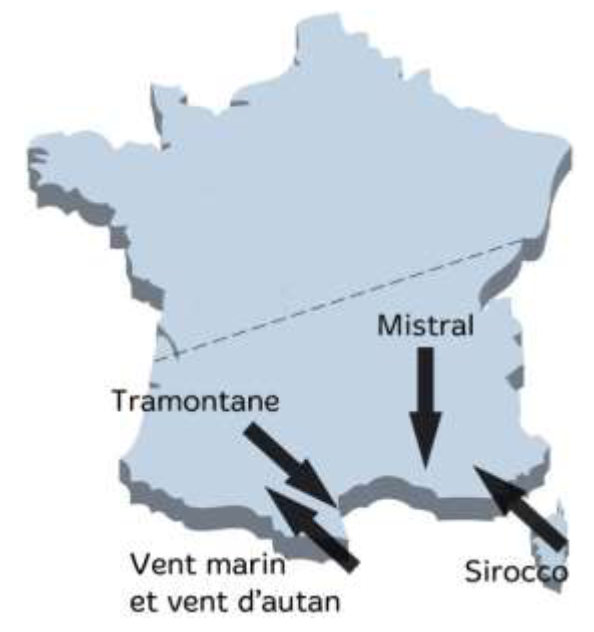
\includegraphics[scale=1]{images/vents.png}
  \end{figure}
\end{frame}

\section{Le vent de travers}

\begin{frame}{Le vent de travers}
  Un avion essaye toujours de se poser face au vent.

  Parfois le vent n'est pas aligné avec la piste, il a une composante de vent de travers.

\end{frame}

\begin{frame}{Atterrissage vent de travers}
  \begin{figure}
    \centering
    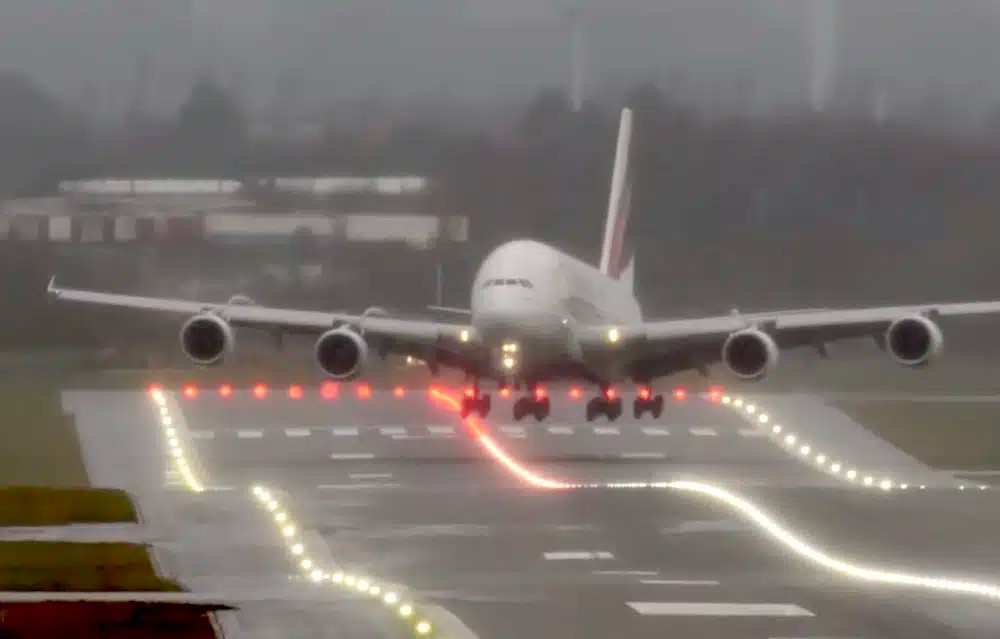
\includegraphics[scale=0.3]{images/A380-atterrissage-travers-CE.jpg}
  \end{figure}
\end{frame}


\begin{frame}{Risque du vent de travers}
  \begin{itemize}
    \item Arrondir hors de la piste \pause
    \item Casser le train car atterrissage en crabe \pause
    \item Vitesse de vent de travers démontrée lors de la certification.
  \end{itemize}
\end{frame}

\begin{frame}{Risque de l'arrondi par vent de travers}
  \begin{figure}
    \centering
    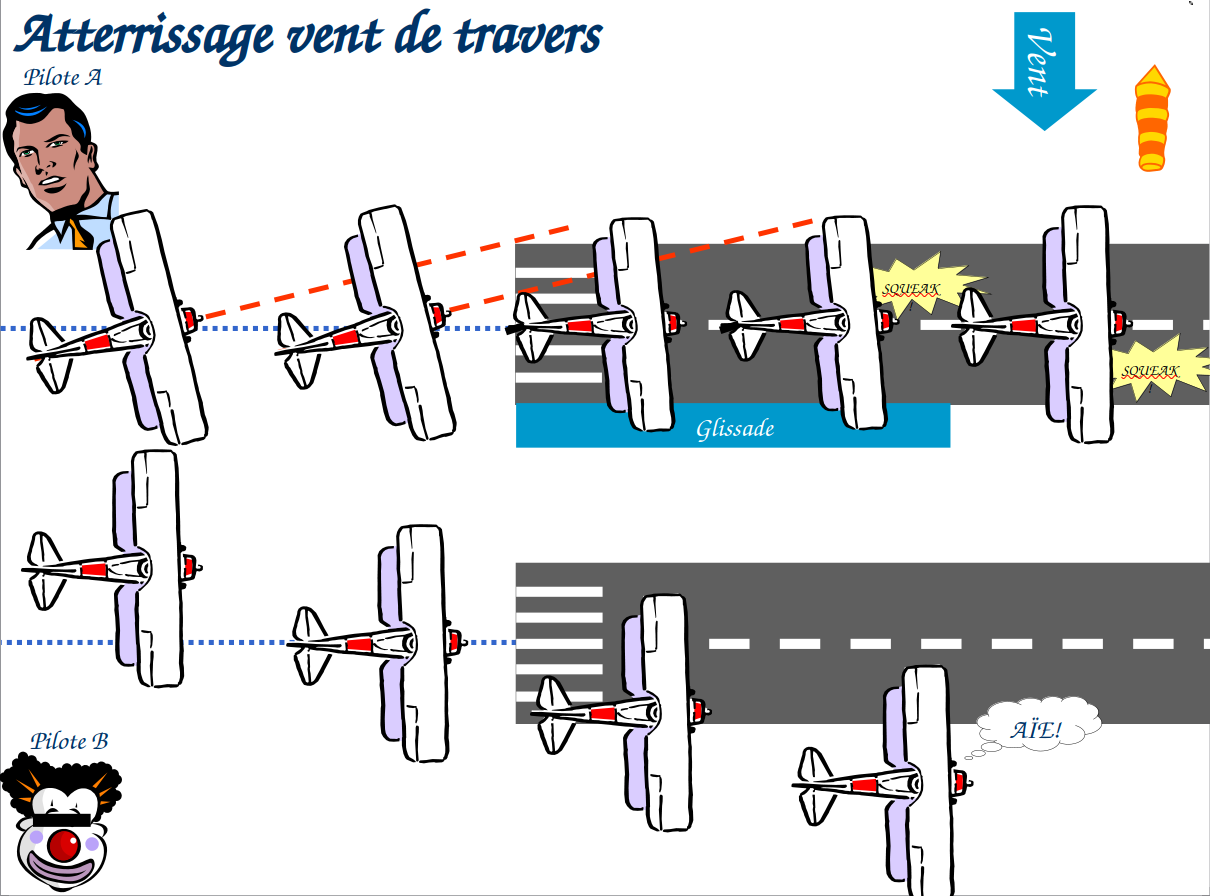
\includegraphics[scale=0.9]{images/vent-travers.png}
  \end{figure}
\end{frame}

\begin{frame}{Estimation de la composante de vent de travers avec le LOC}
  \begin{figure}
    \centering
    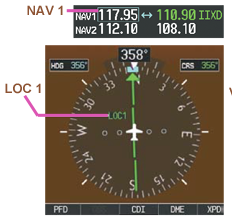
\includegraphics[scale=0.8]{images/loc.png}
  \end{figure}
\end{frame}

\begin{frame}{Estimation de la composante de vent de travers — Règle des tiers}
  \begin{figure}
    \centering
    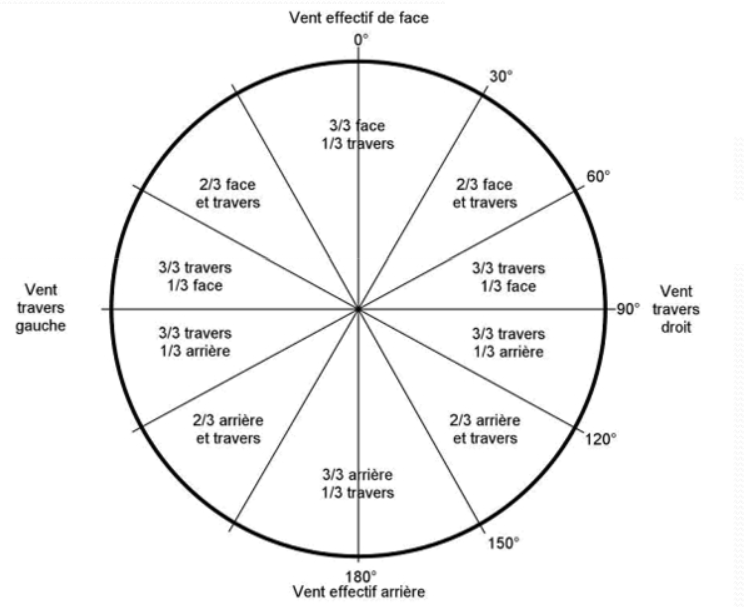
\includegraphics[scale=1.2]{images/tiers.png}
  \end{figure}
\end{frame}

\end{document}
